% Гайд к лабораторной работе №2 (BCR::ABL1: структуры WT и T315I)
% Компиляция: pdflatex guide.tex  (дважды, из папки guide)
\documentclass[12pt,a4paper]{article}

\usepackage{cmap}
\usepackage[T2A]{fontenc}
\usepackage[utf8]{inputenc}
\usepackage[russian]{babel}
\usepackage[left=2.5cm,right=1.5cm,top=2cm,bottom=2cm]{geometry}
\usepackage{booktabs}
\usepackage{longtable}
\usepackage{array}
\usepackage{graphicx}
\usepackage{enumitem}
\usepackage{amsmath}
\usepackage{float}
\usepackage{caption}
\usepackage{listings}
\usepackage[hidelinks]{hyperref}
\usepackage[expansion=false]{microtype}

\captionsetup{font=small,labelfont=bf}
\setlength{\parindent}{1.25em}
\setlength{\emergencystretch}{3em}
\renewcommand{\arraystretch}{1.2}

\newcolumntype{L}[1]{>{\raggedright\arraybackslash}p{#1}}
\newcommand{\code}[1]{{\ttfamily #1}}

\lstset{
  basicstyle=\ttfamily\small,
  breaklines=true,
  frame=single,
  framesep=4pt,
  rulecolor=\color{black},
  columns=flexible,
  showstringspaces=false,
}
\usepackage{color}

\title{\textbf{Гайд к лабораторной работе №2}\\[4pt]
Экспериментальные структуры белка: как их читать, проверять и готовить к докингу\\[4pt]
\large На примере киназного домена ABL1: 2HYY (WT) и 3QRJ (T315I)}
\author{Шпока Владислав, Пясецкий Кирилл\\4 курс, 3 группа}
\date{4 октября 2026 г.}

\begin{document}
\maketitle
\tableofcontents
\newpage

\section{Зачем вообще нужна эта работа}

В первой лабораторной мы выяснили, \emph{что} является мишенью: белок ABL1
(UniProt \code{P00519}), его киназный домен 242--493, мутация T315I в
gatekeeper-остатке, и выбрали две структуры --- \textbf{2HYY} для WT и
\textbf{3QRJ} для T315I. Но сами координаты мы тогда не трогали: работали с
аннотациями баз данных.

Вторая работа --- это переход от «записи в базе» к «файлу, с которым можно
считать». Цель: получить из публичной записи PDB такой набор файлов, который
можно подать на вход докингу, и при этом быть уверенным, что мы понимаем, что
именно в этих файлах лежит.

Ключевая мысль работы: \textbf{экспериментальная структура --- это не точная копия
белка, а модель, построенная по электронной плотности}. В ней может не хватать
кусков цепи, могут быть лишние молекулы из буфера, нумерация может не совпадать с
UniProt, а «тот же самый белок» в двух записях может выглядеть по-разному из-за
разных лигандов. Всё это нужно проверить руками до того, как запускать расчёты.

\section{Теория: что такое PDB-структура}

\subsection{Откуда берутся координаты}

Подавляющее большинство структур белков получено \textbf{рентгеновской
дифракцией} (X-ray diffraction). Схема такая:

\begin{enumerate}[leftmargin=*,topsep=2pt,itemsep=3pt]
\item Белок очищают и заставляют кристаллизоваться --- образовать регулярную
трёхмерную решётку из миллионов одинаково ориентированных молекул.
\item Кристалл облучают рентгеном. Электроны атомов рассеивают излучение, и из-за
регулярности решётки рассеянные волны интерферируют: на детекторе появляется набор
дискретных рефлексов.
\item По интенсивностям рефлексов восстанавливают \textbf{карту электронной
плотности} --- трёхмерную функцию «где в ячейке много электронов».
\item В эту карту \emph{вписывают} модель: исследователь (и программа) размещают
атомы так, чтобы они объясняли наблюдаемую плотность.
\end{enumerate}

Последний пункт принципиален: координаты в PDB-файле --- это \emph{интерпретация}
плотности, а не прямое измерение положения каждого атома.

\subsection{Разрешение и что оно значит}

\textbf{Разрешение} (resolution, в ангстремах) --- минимальное расстояние, на
котором две детали карты ещё различимы. Чем меньше число, тем лучше:

\begin{center}
\begin{tabular}{L{3.0cm}L{11.5cm}}
\toprule
\textbf{Разрешение} & \textbf{Что видно} \\
\midrule
лучше 1{,}5~\AA & Отдельные атомы, альтернативные конформации боковых цепей, много
упорядоченной воды \\
1{,}5--2{,}0~\AA & Боковые цепи уверенно различимы, положение лиганда надёжно ---
\emph{хороший уровень для докинга} \\
2{,}0--2{,}5~\AA & Основная цепь надёжна, некоторые боковые цепи на поверхности
неоднозначны \\
хуже 3{,}0~\AA & Виден в основном ход цепи; детали карманов ненадёжны \\
\bottomrule
\end{tabular}
\end{center}

Наши структуры: 2HYY --- 2{,}40~\AA{} (приемлемо), 3QRJ --- 1{,}82~\AA{} (хорошо).
Именно поэтому в 3QRJ разрешено в 2{,}5 раза больше молекул воды, хотя цепей
меньше: при лучшем разрешении различимо больше упорядоченного растворителя.

\subsection{B-фактор}

У каждого атома в файле есть \textbf{B-фактор} (temperature factor) --- мера
«размазанности» атома по карте плотности. Высокий B означает, что атом подвижен или
его положение определено плохо. В нашем примере у N-концевого Trp235 B-фактор
равен 89 --- это очень много, типично для края конструкции, который болтается.
У атомов в глубине кармана B обычно 15--30.

Практический смысл: если остаток сайта связывания имеет B-фактор под 80, доверять
его точной геометрии не стоит.

\subsection{Почему в структуре не хватает кусков}

Если участок цепи подвижен (петля, не зафиксированная контактами), он не даёт
регулярного вклада в плотность --- плотности там просто нет, и вписать атомы
некуда. Такие остатки в файл не попадают: в последовательности они есть, а
координат у них нет. Это и есть \textbf{missing residues}, пропуски.

Важное следствие: \textbf{нумерация остатков не непрерывна}. После остатка 273
может сразу идти 279. Если наивно пройтись по файлу подряд, можно «склеить»
несоседние остатки.

\subsection{Что ещё лежит в файле, кроме белка}

\begin{itemize}[leftmargin=*,topsep=2pt,itemsep=2pt]
\item \textbf{Лиганд} --- интересующая нас малая молекула (ингибитор). У неё есть
трёхсимвольный код химического компонента: \code{STI} --- иматиниб,
\code{919} --- ребастиниб.
\item \textbf{Вода} (\code{HOH}) --- упорядоченные молекулы растворителя.
\item \textbf{Ионы и добавки} --- Na$^+$, Mg$^{2+}$, Ni$^{2+}$, глицерин, сульфат:
попадают из буфера кристаллизации. В наших структурах их нет.
\item \textbf{Несколько копий белка} --- в асимметричной ячейке может быть
несколько молекул (в 2HYY --- четыре цепи A, B, C, D). Это кристаллографическая
особенность, а не биологический тетрамер.
\end{itemize}

\subsection{Формат ATOM-записи}

Классический PDB --- формат с \emph{фиксированными колонками}: смысл поля
определяется его позицией в строке, а не разделителем.

\begin{lstlisting}
ATOM      1  N   TRP A 235       2.281   3.258  18.672  1.00 89.25           N
\end{lstlisting}

\begin{center}
\begin{tabular}{L{2.2cm}L{3.6cm}L{8.4cm}}
\toprule
\textbf{Колонки} & \textbf{Поле} & \textbf{Пояснение} \\
\midrule
1--6 & тип записи & \code{ATOM} --- полимер, \code{HETATM} --- всё остальное \\
7--11 & номер атома & сквозная нумерация по файлу \\
13--16 & имя атома & \code{N}, \code{CA}, \code{CB}, \code{OG1}\ldots \\
18--20 & имя остатка & трёхбуквенный код \\
22 & цепь & \code{A} \\
23--26 & номер остатка & \textbf{в системе нумерации записи} \\
31--38 & X & ангстремы \\
39--46 & Y & \\
47--54 & Z & \\
55--60 & occupancy & доля конформации (1.00 --- единственная) \\
61--66 & B-фактор & подвижность \\
77--78 & элемент & \code{N}, \code{C}, \code{O}, \code{S} \\
\bottomrule
\end{tabular}
\end{center}

Современный формат --- \textbf{mmCIF} (\code{.cif}): это таблицы «ключ--значение»
без ограничения на ширину поля. PDB-формат ломается на структурах с числом атомов
больше 99999 или числом цепей больше 62, поэтому RCSB считает mmCIF основным.
Мы скачиваем \code{.cif}, а рабочие файлы сохраняем в \code{.pdb}, потому что
программы докинга чаще ждут именно его.

\section{Теория: нумерация остатков --- главный источник ошибок}

\subsection{Откуда берётся расхождение}

Номер остатка в PDB-файле --- это то, что авторы структуры написали в своей статье.
Он не обязан совпадать с позицией в канонической последовательности UniProt.
Причины расхождений:

\begin{enumerate}[leftmargin=*,topsep=2pt,itemsep=3pt]
\item \textbf{Разные изоформы.} У ABL1 есть изоформа 1a (1130 а.о.,
\code{P00519-1}) и 1b (на 19 остатков длиннее). Один и тот же gatekeeper в первой
нумерации --- Thr315, во второй --- Thr334. В литературе встречаются обе; запись
\code{5MO4} из первой лабораторной, например, обозначает мутацию как \code{T334I}.
\item \textbf{Другой организм.} Мышиный ортолог (\code{P00520}) имеет свою
нумерацию.
\item \textbf{Искусственные конструкции.} Если белок экспрессировали с меткой
(His-tag), авторы иногда нумеруют с учётом метки.
\end{enumerate}

\subsection{Как проверять, а не угадывать}

Нельзя полагаться на то, что «остаток 315 --- это Thr315». Нужно сопоставить
\emph{последовательность}. Надёжный способ, использованный в работе: перебрать все
возможные сдвиги и посмотреть, при каком из них последовательность структуры лучше
всего ложится на последовательность UniProt.

\begin{lstlisting}[language=Python]
# for each candidate shift, count how many residues match UniProt
best = (0, -1.0)
for offset in range(-40, 41):
    hit = total = 0
    for num, name in residues:          # (seqid, 3-letter name) from the chain
        pos = num + offset
        if 1 <= pos <= len(useq):
            total += 1
            if one_letter(name) == useq[pos - 1]:
                hit += 1
    if total and hit / total > best[1]:
        best = (offset, hit / total)
\end{lstlisting}

Результат для наших структур: сдвиг \textbf{0} для обеих. Доля совпадений 100\,\%
для 2HYY и 99{,}6\,\% для 3QRJ.

\medskip
\noindent\textbf{Почему 99{,}6\,\%, а не 100\,\%} --- это не ошибка, а проверка.
Единственное несовпадение в 3QRJ приходится ровно на остаток 315: в UniProt там
\code{T}, в структуре \code{I}. Мутация честно проявилась как одно расхождение.
Заодно это доказывает, что \emph{других} замен в структуре нет: будь их больше,
несовпадений было бы больше одного.

\section{Теория: наложение структур и RMSD}

\subsection{Что считает Matchmaker}

Чтобы сравнить две структуры, их нужно привести в одну систему координат. Задача:
найти поворот $R$ и сдвиг $\mathbf{t}$, минимизирующие сумму квадратов расстояний
между соответственными атомами. Это классическая \textbf{задача Кабша}, решаемая
через сингулярное разложение:

\begin{enumerate}[leftmargin=*,topsep=2pt,itemsep=2pt]
\item Совместить центры масс обоих наборов точек.
\item Построить ковариационную матрицу $H = P^{\mathsf T} Q$.
\item Разложить $H = U \Sigma V^{\mathsf T}$; тогда $R = V D U^{\mathsf T}$, где
$D = \mathrm{diag}(1, 1, \mathrm{sign}\det(VU^{\mathsf T}))$ --- поправка,
запрещающая зеркальное отражение.
\end{enumerate}

Мера качества --- \textbf{RMSD} (root-mean-square deviation):
\[
\mathrm{RMSD} = \sqrt{\frac{1}{N}\sum_{i=1}^{N} \lVert \mathbf{p}_i - \mathbf{q}_i \rVert^2 }
\]
То есть среднеквадратичное расстояние между парами соответственных атомов после
наилучшего совмещения. Обычно считают по C$\alpha$ --- по одному опорному атому
на остаток.

\subsection{Как строятся пары остатков}

ChimeraX по умолчанию (\code{pairing ss}) сначала выравнивает последовательности с
учётом вторичной структуры, и уже потом совмещает. Это нужно, когда нумерации
разные или белки разные.

В нашем случае проверено, что нумерации обеих структур совпадают с UniProt, поэтому
в скрипте пары строятся прямо по номерам остатков. Это точнее: исключается риск,
что алгоритм выравнивания сместит рамку на похожем участке.

\subsection{Итеративное отбрасывание и почему RMSD два}

Одна подвижная петля может испортить всё наложение: алгоритм «тянет» оптимум, чтобы
уменьшить её огромный вклад, и портит совмещение хорошо совпадающей части.
Поэтому Matchmaker делает \textbf{iterative pruning}:

\begin{enumerate}[leftmargin=*,topsep=2pt,itemsep=2pt]
\item Совместить по всем парам, посчитать отклонения.
\item Выбросить пары с отклонением больше порога (по умолчанию 2{,}0~\AA).
\item Совместить заново по оставшимся. Повторять до стабилизации.
\end{enumerate}

В журнале появляются \emph{два} числа: RMSD по всем парам и RMSD по оставшимся.
Оба нужно записать --- вместе они говорят больше, чем по отдельности. Большая
разница между ними означает: «основная часть совпадает отлично, но есть локальные
участки сильного расхождения».

\section{Что именно сделано в работе, шаг за шагом}

\subsection{Инструменты}

Задание написано под UCSF ChimeraX. На рабочей машине его нет, и поставить его в
Python-окружение нельзя: ChimeraX --- настольное приложение со своим
интерпретатором, в PyPI его нет. Поэтому все операции выполнены через библиотеку
\code{gemmi} (чтение mmCIF/PDB, работа с моделями и цепями) и \code{numpy}
(линейная алгебра наложения), а в отчёте для каждого шага приведена эквивалентная
команда ChimeraX.

Это не упрощение: все числа получены из тех же координат, которые прочитал бы
ChimeraX, а наложение воспроизводит именно алгоритм Matchmaker, включая итеративное
отбрасывание.

\subsection{Шаг 1. Загрузка}

Структуры скачаны напрямую с RCSB:

\begin{lstlisting}
https://files.rcsb.org/download/2HYY.cif
https://files.rcsb.org/download/3QRJ.cif
\end{lstlisting}

и сохранены как \code{WT\_original.cif} и \code{T315I\_original.cif}.

\subsection{Шаг 2. Выбор цепи}

В 2HYY четыре цепи (A--D), в 3QRJ две (A, B). Все цепи в каждой структуре --- один
и тот же белок (одна полимерная сущность). Взята цепь \code{A} в обеих.

\medskip
\noindent\emph{Почему именно A и почему вообще одна.} Несколько цепей --- это
кристаллографическая копия, а не биологический комплекс: киназный домен ABL1
функционирует как мономер. Брать все четыре копии в докинг бессмысленно --- это
учетверит расчёт без новой информации. Цепь A выбрана как первая и, в 2HYY,
наиболее полная.

\subsection{Шаг 3. Проверка полноты}

\begin{center}
\begin{tabular}{L{4.6cm}L{4.9cm}L{4.9cm}}
\toprule
 & \textbf{2HYY, цепь A} & \textbf{3QRJ, цепь A} \\
\midrule
Разрешено остатков & 263 & 258 \\
Диапазон & 235--498 & 234--496 \\
Внутренние пропуски & 275 (1 остаток) & 274--278 (5 остатков) \\
Пропуски в сайте связывания & нет & нет \\
\bottomrule
\end{tabular}
\end{center}

Пропуски попадают в границы киназного домена (242--493), но лежат в петле между
$\beta$3 и $\alpha$C --- она выходит на поверхность и в формировании кармана не
участвует. Это проверено не на глаз: скрипт считает список остатков в радиусе
4{,}5~\AA{} от лиганда и сверяет его с границами пропусков. Ни один контактный
остаток не потерян.

\subsection{Шаг 4. Поиск остатка 315 и проверка нумерации}

Найдено: \code{THR 315} в 2HYY, \code{ILE 315} в 3QRJ, сдвиг нумерации 0 для обеих
(см. раздел~3). Мутация присутствует в координатах, а не только в аннотации.

\subsection{Шаг 5. Лиганд и сайт связывания}

\begin{center}
\begin{tabular}{L{4.8cm}L{4.8cm}L{4.8cm}}
\toprule
 & \textbf{2HYY} & \textbf{3QRJ} \\
\midrule
Ингибитор & иматиниб & ребастиниб (DCC-2036) \\
Код компонента & \code{STI} & \code{919} \\
Атомов (без H) & 37 & 41 \\
Контактных остатков ($\le 4{,}5$~\AA) & 25 & 27 \\
\bottomrule
\end{tabular}
\end{center}

В обоих списках контактов присутствуют: остаток \textbf{315} (Thr или Ile),
каталитический \textbf{Lys271}, шарнирные \textbf{Glu316--Phe317--Met318} и мотив
\textbf{DFG} (Asp381--Phe382--Gly383). Это стандартный набор для ATP-кармана
киназы --- подтверждение, что лиганд сидит там, где ожидается, и что остаток 315
действительно образует стенку кармана, а не просто находится поблизости.

\subsection{Шаг 6. Сохранение рабочих файлов}

Для каждой формы сохранено по два файла:

\begin{center}
\begin{tabular}{L{5.2cm}L{4.4cm}L{2.2cm}L{2.0cm}}
\toprule
\textbf{Файл} & \textbf{Содержимое} & \textbf{Остатков} & \textbf{Атомов} \\
\midrule
\code{WT\_complex.pdb} & цепь A + иматиниб & 264 & 2110 \\
\code{WT\_protein.pdb} & цепь A, белок & 263 & 2073 \\
\code{T315I\_complex.pdb} & цепь A + ребастиниб & 259 & 2116 \\
\code{T315I\_protein.pdb} & цепь A, белок & 258 & 2075 \\
\bottomrule
\end{tabular}
\end{center}

\noindent\emph{Зачем два варианта.} Файл «белок + лиганд» нужен для
\textbf{редокинга}: мы знаем экспериментальную позу ингибитора, запускаем докинг и
смотрим, воспроизводит ли программа эту позу. Если да --- протоколу можно доверять.
Файл «только белок» --- это приёмник (receptor) для докинга новых молекул.

\noindent\emph{Почему без воды.} Кристаллографическая вода в кармане --- отдельная
большая тема. Часть молекул воды структурно важна (опосредует водородные связи),
часть --- случайна. Стандартная практика --- убирать воду и при необходимости
возвращать отдельные молекулы осознанно. Поэтому в рабочих файлах воды нет.

\subsection{Шаг 7. Наложение}

\begin{center}
\begin{tabular}{L{8.6cm}L{5.9cm}}
\toprule
\textbf{Показатель} & \textbf{Значение} \\
\midrule
Пар остатков (общие номера) & 257 \\
RMSD по всем парам & 1{,}292~\AA \\
Итераций отбрасывания (порог 2{,}0~\AA) & 4 \\
Пар после отбрасывания & 242 \\
RMSD после отбрасывания & \textbf{0{,}815~\AA} \\
RMSD внутри киназного домена & 1{,}301~\AA{} (247 пар) \\
RMSD около остатка 315 ($\pm 5$) & 0{,}920~\AA{} (11 пар) \\
Отклонение C$\alpha$ остатка 315 & 0{,}386~\AA \\
\bottomrule
\end{tabular}
\end{center}

\section{Главный результат и как его интерпретировать}

\subsection{Структуры почти одинаковы}

0{,}815~\AA{} по 242 парам --- это уровень совпадения двух кристаллических форм
одного и того же белка. Для сравнения: разные белки одного семейства дают
2--4~\AA, а разные конформации одной киназы (DFG-in против DFG-out) --- порядка
1{,}5--3~\AA. Значит, замена Thr$\rightarrow$Ile \textbf{не перестраивает укладку}
киназного домена.

\subsection{Но различия есть, и они не там, где мутация}

\begin{figure}[H]
\centering
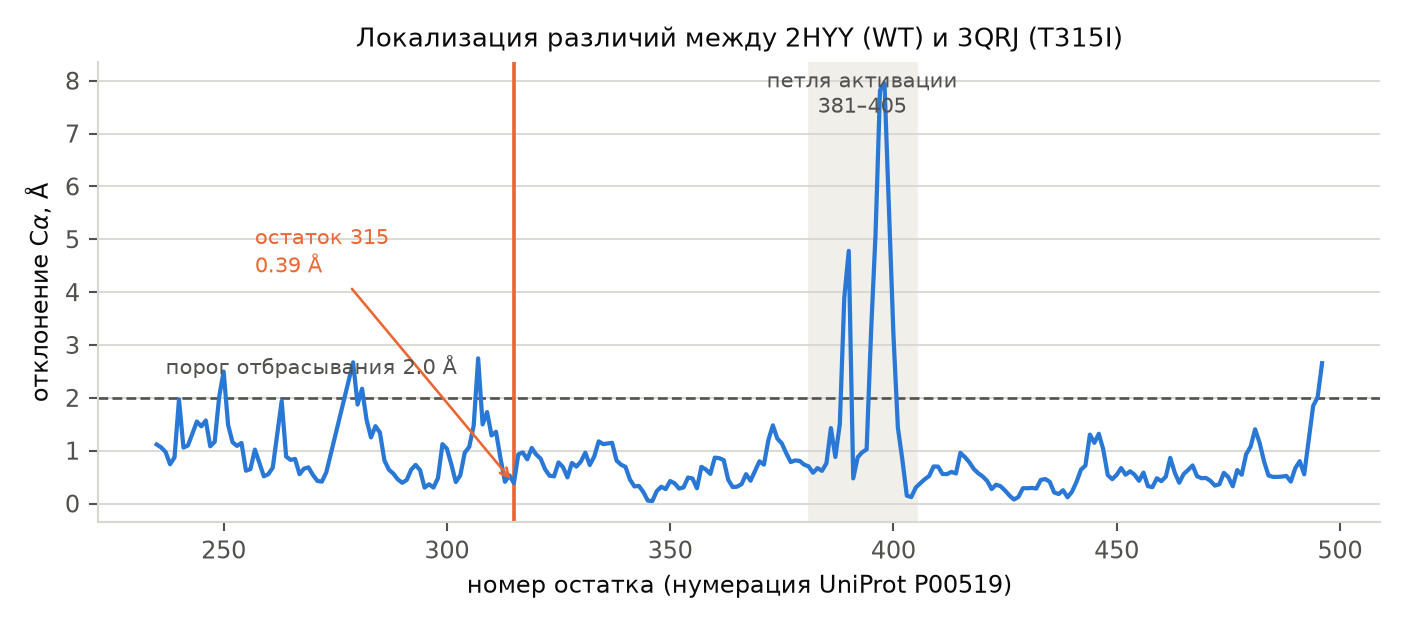
\includegraphics[width=\linewidth]{../figures/fig_deviation.png}
\caption{Отклонение C$\alpha$ по остаткам после наложения. Почти везде меньше
1~\AA; выброс до 8~\AA{} --- остатки 389--400, то есть петля активации (381--405).
В позиции 315 отклонение минимально (0{,}386~\AA).}
\end{figure}

Наибольшие расхождения: остаток 398 --- 7{,}95~\AA, 397 --- 7{,}82~\AA,
399 --- 5{,}59~\AA, 396 --- 5{,}10~\AA, 390 --- 4{,}78~\AA. Все они лежат в петле
активации 381--405 (границы взяты из UniProt, результат лабораторной №1).

\medskip
\noindent\textbf{Почему расходится именно петля активации.} Это подвижный
регуляторный элемент киназы: в активной конформации она развёрнута и формирует
площадку для субстрата, в неактивной --- сложена внутрь и блокирует карман. Её
положение определяется тем, какой лиганд связан и в каких условиях рос кристалл.
В 2HYY связан иматиниб (стабилизирует неактивную DFG-out конформацию), в 3QRJ ---
ребастиниб, другая молекула с другим способом связывания. То есть \emph{крупнейшее
различие между структурами вызвано разными лигандами, а не мутацией T315I}.

Это важно честно проговорить: мы сравниваем не «WT против T315I в одинаковых
условиях», а две разные кристаллические структуры, которые отличаются сразу по двум
параметрам --- и мутацией, и связанным ингибитором. Разделить эти два вклада по
имеющимся данным нельзя.

\subsection{Почему глобальное RMSD обманчиво}

\begin{figure}[H]
\centering
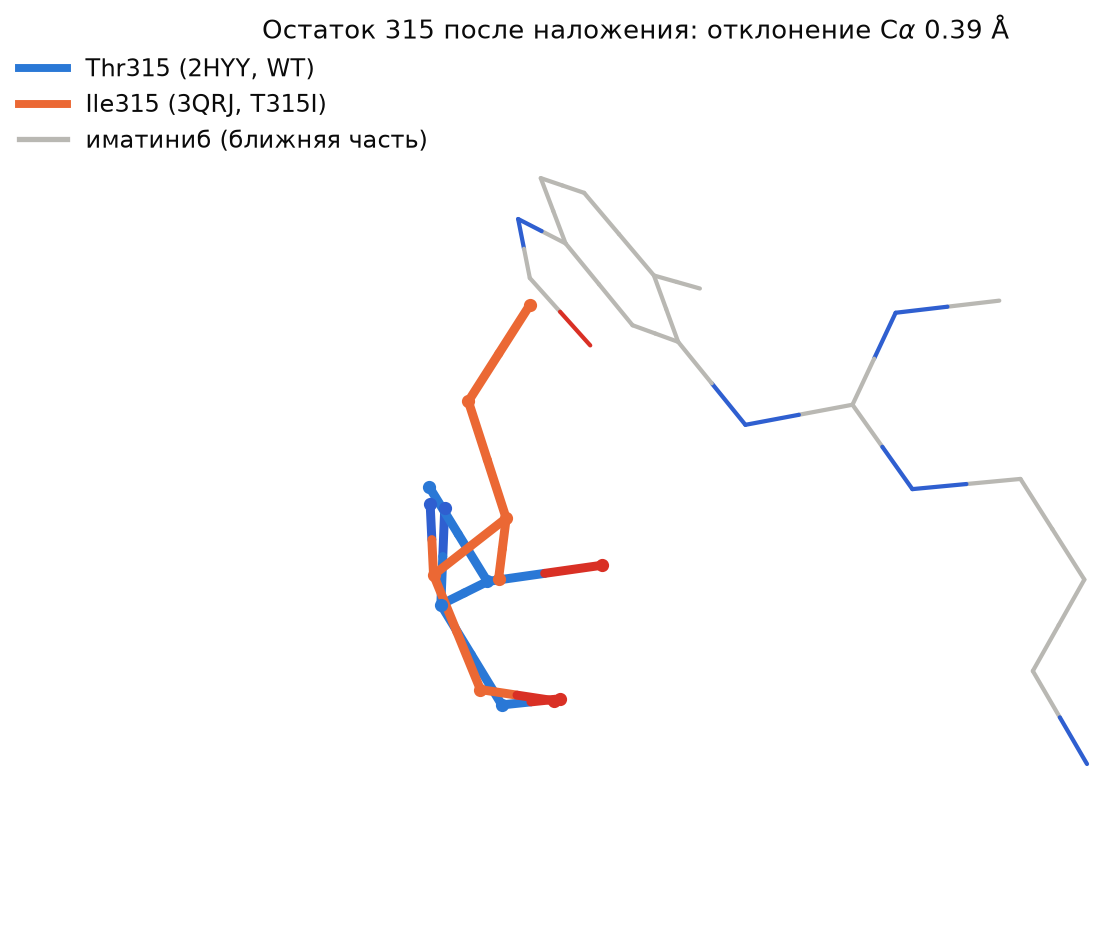
\includegraphics[width=0.85\linewidth]{../figures/fig_315_overlay.png}
\caption{Thr315 и Ile315 после наложения. Основная цепь совпадает, но боковая цепь
изолейцина разветвлена и уходит дальше в сторону кармана.}
\end{figure}

Три причины, по которым «RMSD 0{,}8~\AA» не означает «карманы одинаковые»:

\begin{enumerate}[leftmargin=*,topsep=2pt,itemsep=3pt]
\item \textbf{Усреднение.} RMSD считается по 257 парам. Вклад одного остатка ---
порядка $\sqrt{1/257}\approx 6\,\%$; локальное изменение в нём просто растворяется.
\item \textbf{Считается по C$\alpha$, а меняется боковая цепь.} Отклонение
C$\alpha$ остатка 315 --- 0{,}386~\AA, то есть \emph{меньше} среднего по структуре.
С точки зрения основной цепи «ничего не произошло». А объём боковой цепи вырос со
$\approx$116 до $\approx$167~\AA$^3$ --- именно это закрывает вход в гидрофобный
карман и убирает донор водородной связи.
\item \textbf{Самое большое различие не связано с вопросом.} Петля активации
расходится на 8~\AA{} и формирует почти весь глобальный RMSD, хотя к механизму
резистентности отношения не имеет.
\end{enumerate}

\noindent\textbf{Практический вывод:} для оценки сайта связывания нужны локальные
метрики --- объём кармана, список контактов, геометрия водородных связей, --- а не
одно число по всей структуре.

\section{Разбор кода}

\subsection{Структура проекта}

\begin{center}
\begin{tabular}{L{5.6cm}L{8.9cm}}
\toprule
\textbf{Файл} & \textbf{Что делает} \\
\midrule
\code{scripts/}\allowbreak\code{prepare\_structures.py} & читает \code{.cif},
определяет цепь, пропуски, нумерацию, лиганд, сайт связывания; сохраняет шесть
рабочих файлов \\
\code{scripts/}\allowbreak\code{superpose.py} & наложение Кабша, итеративное
отбрасывание, RMSD \\
\code{scripts/}\allowbreak\code{make\_figures.py} & иллюстрации по координатам \\
\code{data/analysis.json} & все числа первого скрипта \\
\code{data/superposition.json} & все числа второго, включая отклонение по каждому
остатку \\
\bottomrule
\end{tabular}
\end{center}

\subsection{Поиск пропусков}

Пропуск --- это разрыв в нумерации подряд идущих разрешённых остатков:

\begin{lstlisting}[language=Python]
def find_gaps(residues):
    # residues is a sorted list of (seqid, resname)
    gaps = []
    for (n1, _), (n2, _) in zip(residues, residues[1:]):
        if n2 > n1 + 1:
            gaps.append((n1 + 1, n2 - 1))
    return gaps
\end{lstlisting}

\subsection{Остатки сайта связывания}

Для каждого остатка белка ищем минимальное расстояние до любого атома лиганда:

\begin{lstlisting}[language=Python]
def contact_residues(chain, ligand, cutoff):
    lig_pos = [atom.pos for atom in ligand]
    hits = []
    for res in chain:
        best = None
        for atom in res:
            for lp in lig_pos:
                d = atom.pos.dist(lp)
                if best is None or d < best:
                    best = d
        if best is not None and best <= cutoff:
            hits.append((res.seqid.num, res.name, round(best, 2)))
    return hits
\end{lstlisting}

Порог 4{,}5~\AA{} --- стандартный для «первой координационной сферы»: он
захватывает водородные связи (2{,}6--3{,}2~\AA) и ван-дер-ваальсовы контакты
(3{,}4--4{,}2~\AA), но не притягивает далёкие остатки.

\subsection{Наложение Кабша}

\begin{lstlisting}[language=Python]
def kabsch(P, Q):
    pc, qc = P.mean(axis=0), Q.mean(axis=0)
    H = (P - pc).T @ (Q - qc)
    U, _, Vt = np.linalg.svd(H)
    d = np.sign(np.linalg.det(Vt.T @ U.T))   # forbid reflection
    D = np.diag([1.0, 1.0, d])
    R = Vt.T @ D @ U.T
    return R, qc - R @ pc
\end{lstlisting}

Строка с \code{d} существенна: без неё SVD может выдать матрицу с определителем
$-1$, то есть зеркальное отражение. Оно формально уменьшило бы RMSD, но
соответствовало бы физически невозможной (зеркальной) молекуле.

\subsection{Итеративное отбрасывание}

\begin{lstlisting}[language=Python]
keep = np.ones(len(common), dtype=bool)
for it in range(1, 21):
    R, t = kabsch(P[keep], Q[keep])
    P_fit = (R @ P.T).T + t
    dev = np.linalg.norm(P_fit - Q, axis=1)
    new_keep = dev <= PRUNE_CUTOFF
    if new_keep.sum() < 3 or (new_keep == keep).all():
        break
    keep = new_keep
\end{lstlisting}

Выход из цикла --- когда набор перестал меняться (сошлось) или когда пар осталось
слишком мало. У нас сошлось за 4 итерации: 257 пар $\rightarrow$ 242.

\section{Как повторить всё с нуля}

\begin{lstlisting}
cd d:\uni\karpenka_labs\lab2

# 1. download structures (2HYY, 3QRJ) into structures/
curl -o structures/2hyy.cif https://files.rcsb.org/download/2HYY.cif
curl -o structures/3qrj.cif https://files.rcsb.org/download/3QRJ.cif

# 2. analyse and build the six working files
..\.venv\Scripts\python.exe scripts\prepare_structures.py

# 3. superposition and RMSD
..\.venv\Scripts\python.exe scripts\superpose.py

# 4. figures
..\.venv\Scripts\python.exe scripts\make_figures.py

# 5. documents (twice each)
cd report && pdflatex report.tex && pdflatex report.tex
cd ..\guide && pdflatex guide.tex && pdflatex guide.tex
\end{lstlisting}

Окружение --- общий venv лабораторных \code{karpenka\_labs/.venv} (Python 3.14;
\code{gemmi}, \code{numpy}, \code{matplotlib}, \code{requests}, \code{openpyxl}).
Первый скрипт читает \code{lab1/}\allowbreak\code{data/}\allowbreak\code{uniprot\_P00519.json}, поэтому папка \code{lab1}
должна лежать рядом.

\medskip
\noindent\textbf{Если делать в ChimeraX.} Последовательность команд приведена в
отчёте для каждого пункта. Полный сценарий:

\begin{lstlisting}
open WT_original.cif
info #1
cartoon #1/A
hide #1/A atoms
select #1/A:315
show sel atoms
style sel stick
select #1:STI
show sel atoms
style sel stick
select clear
select (#1/A & protein) | (#1:STI)
save WT_complex.pdb models #1 selectedOnly true
select clear
select #1/A & protein
save WT_protein.pdb models #1 selectedOnly true
close session
open WT_original.cif
open T315I_original.cif
matchmaker #2/A to #1/A pairing ss
select #1/A:315 | #2/A:315
show sel atoms
style sel stick
\end{lstlisting}

Для T315I те же команды с заменой \code{STI} на \code{919} и имён файлов.

\section{Честные ограничения работы}

\begin{enumerate}[leftmargin=*,topsep=2pt,itemsep=3pt]
\item \textbf{Сравниваются структуры с разными лигандами.} 2HYY содержит иматиниб,
3QRJ --- ребастиниб. Поэтому разделить вклад мутации и вклад лиганда в наблюдаемые
различия невозможно. Корректнее было бы сравнивать WT и T315I с одним и тем же
ингибитором, но такой пары среди человеческих структур нет.
\item \textbf{Разные разрешения.} 2{,}40 против 1{,}82~\AA. Часть различий в
положении боковых цепей может объясняться точностью, а не реальной разницей.
\item \textbf{RMSD считался по C$\alpha$.} Это стандарт, но он нечувствителен к
изменениям боковых цепей --- то есть ровно к тому, что составляет суть мутации.
\item \textbf{Межатомные взаимодействия не анализировались.} Водородные связи,
гидрофобные контакты, объём кармана --- предмет следующей работы. Здесь показано
лишь, что остаток 315 входит в сайт связывания.
\item \textbf{Иллюстрации построены не в ChimeraX.} Геометрия в них настоящая
(те же координаты), но это схематичные проволочные представления, а не рендеринг
молекулярного вьюера: нет лент вторичной структуры, поверхностей и освещения.
\item \textbf{Взята одна цепь из нескольких.} Цепи A, B, C, D в 2HYY слегка
различаются; мы не проверяли, насколько выбор цепи A влияет на геометрию кармана.
\end{enumerate}

\section{Вероятные вопросы на защите}

\textbf{Почему для работы берут только киназный домен, а не весь белок?}\\
Полноразмерный BCR::ABL1 ($\approx$2000 а.о. для p210) не закристаллизован.
Патологической является именно киназная активность, и все ATP-конкурентные
ингибиторы связываются в кармане киназного домена. Структурно охарактеризован
только он.

\medskip
\textbf{Что такое gatekeeper и почему он так называется?}\\
Остаток на границе между ATP-карманом и более глубокой гидрофобной полостью
(back pocket). Размер его боковой цепи определяет, пройдёт ли туда ингибитор:
малый Thr оставляет проход открытым, крупный Ile закрывает. Отсюда «привратник».

\medskip
\textbf{Почему в структуре нет части остатков?}\\
Подвижные участки не дают регулярного вклада в электронную плотность, и вписать
туда атомы невозможно. В последовательности они есть, координат нет.

\medskip
\textbf{Почему Matchmaker выдаёт два значения RMSD?}\\
Первое --- по всем парам, второе --- после итеративного отбрасывания пар с
отклонением больше 2~\AA. Большая разница между ними означает, что расхождение
создаётся небольшим числом локальных участков, а не всей структурой. У нас:
1{,}292~\AA{} по 257 парам и 0{,}815~\AA{} по 242.

\medskip
\textbf{RMSD 0{,}8~\AA{} --- значит, структуры идентичны?}\\
Нет. RMSD усредняет по сотням остатков и считается по C$\alpha$. Отклонение
C$\alpha$ остатка 315 --- всего 0{,}386~\AA, хотя именно там находится мутация:
меняется боковая цепь, а не положение основной. Судить о кармане по глобальному
RMSD нельзя.

\medskip
\textbf{Где самые большие различия и почему?}\\
В остатках 389--400 (до 7{,}95~\AA) --- это петля активации 381--405. Её
конформация зависит от связанного лиганда и условий кристаллизации. Поскольку в
двух структурах разные ингибиторы, различие вызвано в первую очередь этим, а не
мутацией.

\medskip
\textbf{Зачем сохранять отдельно «белок» и «белок + лиганд»?}\\
Комплекс --- для редокинга: проверить, воспроизводит ли протокол известную
экспериментальную позу. Только белок --- как приёмник для докинга новых молекул.

\medskip
\textbf{Почему убрали воду?}\\
Часть кристаллографической воды структурно значима, часть случайна, и отличить их
по одной структуре трудно. Стандартная практика --- убрать всю и при необходимости
вернуть отдельные молекулы осознанно.

\medskip
\textbf{Как убедились, что в 3QRJ только одна мутация?}\\
Сопоставлением с последовательностью UniProt: совпало 257 остатков из 258, и
единственное несовпадение --- позиция 315 (\code{T} в UniProt, \code{I} в
структуре). Будь других замен больше, несовпадений было бы больше.

\medskip
\textbf{Чем mmCIF лучше PDB?}\\
PDB --- формат с фиксированной шириной колонок, он ломается при числе атомов
больше 99999 и числе цепей больше 62, и в нём негде хранить расширенные метаданные.
mmCIF --- таблицы без этих ограничений; RCSB считает его основным.

\section{Выводы}

\begin{enumerate}[leftmargin=*,topsep=2pt,itemsep=3pt]
\item Обе выбранные в первой работе структуры пригодны для дальнейшего анализа:
нумерация совпадает с UniProt (сдвиг 0), сайт связывания разрешён полностью,
посторонних мутаций нет, ингибитор присутствует в обеих.
\item Получено шесть рабочих файлов (по три на форму) с прослеживаемой цепочкой
преобразования от записи RCSB.
\item Глобальная укладка WT и T315I совпадает: RMSD 0{,}815~\AA{} по 242 парам
C$\alpha$ после итеративного отбрасывания (1{,}292~\AA{} по всем 257 парам).
\item Мутация не перестраивает укладку: отклонение C$\alpha$ остатка 315 ---
0{,}386~\AA, меньше среднего по структуре.
\item Наибольшие различия (до 7{,}95~\AA) сосредоточены в петле активации 389--400
и объясняются в первую очередь разными связанными лигандами, а не мутацией.
\item Глобальное RMSD не является доказательством идентичности сайта связывания:
оно усредняет по всей цепи и не видит изменений боковых цепей. Для кармана нужны
локальные метрики --- это задача следующей работы.
\end{enumerate}

\end{document}
